\documentclass[twoside]{book}

% Packages required by doxygen
\usepackage{fixltx2e}
\usepackage{calc}
\usepackage{doxygen}
\usepackage[export]{adjustbox} % also loads graphicx
\usepackage{graphicx}
\usepackage[utf8]{inputenc}
\usepackage{makeidx}
\usepackage{multicol}
\usepackage{multirow}
\PassOptionsToPackage{warn}{textcomp}
\usepackage{textcomp}
\usepackage[nointegrals]{wasysym}
\usepackage[table]{xcolor}

% Font selection
\usepackage[T1]{fontenc}
\usepackage[scaled=.90]{helvet}
\usepackage{courier}
\usepackage{amssymb}
\usepackage{sectsty}
\renewcommand{\familydefault}{\sfdefault}
\allsectionsfont{%
  \fontseries{bc}\selectfont%
  \color{darkgray}%
}
\renewcommand{\DoxyLabelFont}{%
  \fontseries{bc}\selectfont%
  \color{darkgray}%
}
\newcommand{\+}{\discretionary{\mbox{\scriptsize$\hookleftarrow$}}{}{}}

% Page & text layout
\usepackage{geometry}
\geometry{%
  a4paper,%
  top=2.5cm,%
  bottom=2.5cm,%
  left=2.5cm,%
  right=2.5cm%
}
\tolerance=750
\hfuzz=15pt
\hbadness=750
\setlength{\emergencystretch}{15pt}
\setlength{\parindent}{0cm}
\setlength{\parskip}{3ex plus 2ex minus 2ex}
\makeatletter
\renewcommand{\paragraph}{%
  \@startsection{paragraph}{4}{0ex}{-1.0ex}{1.0ex}{%
    \normalfont\normalsize\bfseries\SS@parafont%
  }%
}
\renewcommand{\subparagraph}{%
  \@startsection{subparagraph}{5}{0ex}{-1.0ex}{1.0ex}{%
    \normalfont\normalsize\bfseries\SS@subparafont%
  }%
}
\makeatother

% Headers & footers
\usepackage{fancyhdr}
\pagestyle{fancyplain}
\fancyhead[LE]{\fancyplain{}{\bfseries\thepage}}
\fancyhead[CE]{\fancyplain{}{}}
\fancyhead[RE]{\fancyplain{}{\bfseries\leftmark}}
\fancyhead[LO]{\fancyplain{}{\bfseries\rightmark}}
\fancyhead[CO]{\fancyplain{}{}}
\fancyhead[RO]{\fancyplain{}{\bfseries\thepage}}
\fancyfoot[LE]{\fancyplain{}{}}
\fancyfoot[CE]{\fancyplain{}{}}
\fancyfoot[RE]{\fancyplain{}{\bfseries\scriptsize Generated by Doxygen }}
\fancyfoot[LO]{\fancyplain{}{\bfseries\scriptsize Generated by Doxygen }}
\fancyfoot[CO]{\fancyplain{}{}}
\fancyfoot[RO]{\fancyplain{}{}}
\renewcommand{\footrulewidth}{0.4pt}
\renewcommand{\chaptermark}[1]{%
  \markboth{#1}{}%
}
\renewcommand{\sectionmark}[1]{%
  \markright{\thesection\ #1}%
}

% Indices & bibliography
\usepackage{natbib}
\usepackage[titles]{tocloft}
\setcounter{tocdepth}{3}
\setcounter{secnumdepth}{5}
\makeindex

% Hyperlinks (required, but should be loaded last)
\usepackage{ifpdf}
\ifpdf
  \usepackage[pdftex,pagebackref=true]{hyperref}
\else
  \usepackage[ps2pdf,pagebackref=true]{hyperref}
\fi
\hypersetup{%
  colorlinks=true,%
  linkcolor=blue,%
  citecolor=blue,%
  unicode%
}

% Custom commands
\newcommand{\clearemptydoublepage}{%
  \newpage{\pagestyle{empty}\cleardoublepage}%
}

\usepackage{caption}
\captionsetup{labelsep=space,justification=centering,font={bf},singlelinecheck=off,skip=4pt,position=top}

%===== C O N T E N T S =====

\begin{document}

% Titlepage & ToC
\hypersetup{pageanchor=false,
             bookmarksnumbered=true,
             pdfencoding=unicode
            }
\pagenumbering{alph}
\begin{titlepage}
\vspace*{7cm}
\begin{center}%
{\Large My Project }\\
\vspace*{1cm}
{\large Generated by Doxygen 1.8.12}\\
\end{center}
\end{titlepage}
\clearemptydoublepage
\pagenumbering{roman}
\tableofcontents
\clearemptydoublepage
\pagenumbering{arabic}
\hypersetup{pageanchor=true}

%--- Begin generated contents ---
\chapter{Hierarchical Index}
\section{Class Hierarchy}
This inheritance list is sorted roughly, but not completely, alphabetically\+:\begin{DoxyCompactList}
\item Q\+Object\begin{DoxyCompactList}
\item \contentsline{section}{Activity\+Function}{\pageref{class_activity_function}}{}
\end{DoxyCompactList}
\item \contentsline{section}{X\+Neuron}{\pageref{class_x_neuron}}{}
\begin{DoxyCompactList}
\item \contentsline{section}{Gradient\+Training}{\pageref{class_gradient_training}}{}
\item \contentsline{section}{Gradient\+Training2}{\pageref{class_gradient_training2}}{}
\item \contentsline{section}{Online\+Training}{\pageref{class_online_training}}{}
\end{DoxyCompactList}
\end{DoxyCompactList}

\chapter{Class Index}
\section{Class List}
Here are the classes, structs, unions and interfaces with brief descriptions\+:\begin{DoxyCompactList}
\item\contentsline{section}{\hyperlink{class_activity_function}{Activity\+Function} }{\pageref{class_activity_function}}{}
\item\contentsline{section}{\hyperlink{class_gradient_training}{Gradient\+Training} }{\pageref{class_gradient_training}}{}
\item\contentsline{section}{\hyperlink{class_gradient_training2}{Gradient\+Training2} }{\pageref{class_gradient_training2}}{}
\item\contentsline{section}{\hyperlink{class_online_training}{Online\+Training} }{\pageref{class_online_training}}{}
\item\contentsline{section}{\hyperlink{class_x_neuron}{X\+Neuron} }{\pageref{class_x_neuron}}{}
\end{DoxyCompactList}

\chapter{Class Documentation}
\hypertarget{class_activity_function}{}\section{Activity\+Function Class Reference}
\label{class_activity_function}\index{Activity\+Function@{Activity\+Function}}
Inheritance diagram for Activity\+Function\+:\begin{figure}[H]
\begin{center}
\leavevmode
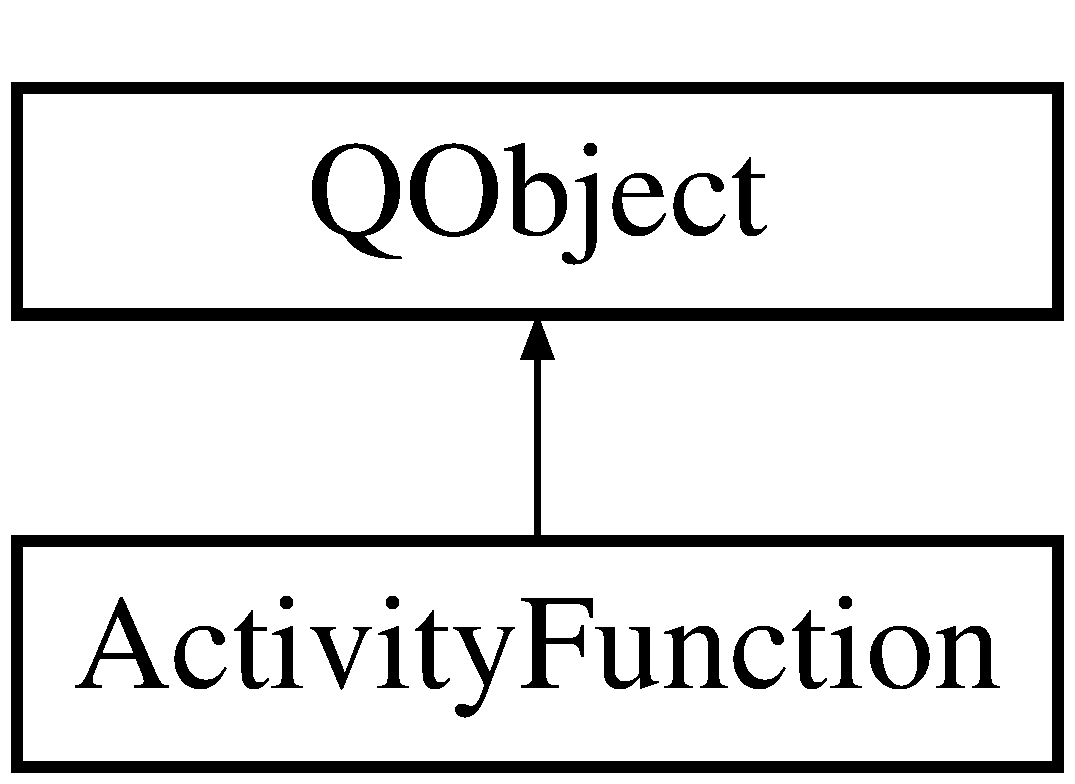
\includegraphics[height=2.000000cm]{class_activity_function}
\end{center}
\end{figure}
\subsection*{Public Types}
\begin{DoxyCompactItemize}
\item 
\hypertarget{class_activity_function_a53d67481011dce859413c787a1ba3ac9}{}\label{class_activity_function_a53d67481011dce859413c787a1ba3ac9} 
enum {\bfseries Act\+Function} \{ \newline
{\bfseries Binary}, 
{\bfseries Line}, 
{\bfseries Line2}, 
{\bfseries Line3}, 
\newline
{\bfseries logistic}, 
{\bfseries Hyperbolic}, 
{\bfseries Normally\+Distributed}
 \}
\end{DoxyCompactItemize}
\subsection*{Public Member Functions}
\begin{DoxyCompactItemize}
\item 
\hypertarget{class_activity_function_ad5ff6526b48659738800209a7c4584ae}{}\label{class_activity_function_ad5ff6526b48659738800209a7c4584ae} 
{\bfseries Activity\+Function} (Q\+Object $\ast$parent)
\end{DoxyCompactItemize}
\subsection*{Static Public Member Functions}
\begin{DoxyCompactItemize}
\item 
\hypertarget{class_activity_function_af2979865b0ed0fdd45f87b794c05bdc7}{}\label{class_activity_function_af2979865b0ed0fdd45f87b794c05bdc7} 
static double {\bfseries give\+Activity\+Function} (Act\+Function func, double out, double bias)
\item 
\hypertarget{class_activity_function_a9750a0424198f685946b3e3b8d3d19b0}{}\label{class_activity_function_a9750a0424198f685946b3e3b8d3d19b0} 
static double {\bfseries Binary\+Func} (double out, double bias)
\item 
\hypertarget{class_activity_function_a3992015d3e75ed3c00590b446271be72}{}\label{class_activity_function_a3992015d3e75ed3c00590b446271be72} 
static double {\bfseries Line\+Func} (double out, double bias, int round)
\item 
\hypertarget{class_activity_function_a13f9b922b9a349b91504fdc5c8606f89}{}\label{class_activity_function_a13f9b922b9a349b91504fdc5c8606f89} 
static double {\bfseries Line2\+Func} (double out, double bias, int round)
\item 
\hypertarget{class_activity_function_a61fdd8afefca23b237685a2f7a303475}{}\label{class_activity_function_a61fdd8afefca23b237685a2f7a303475} 
static double {\bfseries Line3\+Func} (double out, double bias, int round)
\end{DoxyCompactItemize}


The documentation for this class was generated from the following files\+:\begin{DoxyCompactItemize}
\item 
Activity\+Function.\+h\item 
Activity\+Function.\+cpp\end{DoxyCompactItemize}

\hypertarget{class_gradient_training}{}\section{Gradient\+Training Class Reference}
\label{class_gradient_training}\index{Gradient\+Training@{Gradient\+Training}}
Inheritance diagram for Gradient\+Training\+:\begin{figure}[H]
\begin{center}
\leavevmode
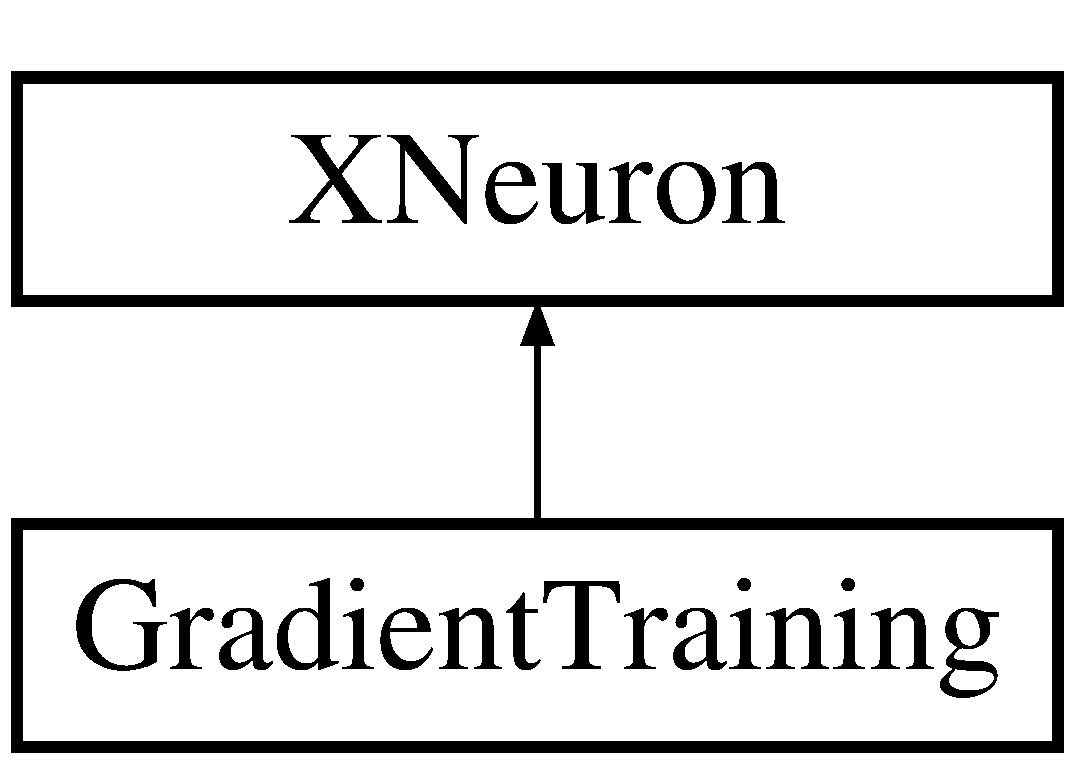
\includegraphics[height=2.000000cm]{class_gradient_training}
\end{center}
\end{figure}
\subsection*{Public Member Functions}
\begin{DoxyCompactItemize}
\item 
\hypertarget{class_gradient_training_ac07db2db785c492f0f1f487703db3c43}{}\label{class_gradient_training_ac07db2db785c492f0f1f487703db3c43} 
bool {\bfseries train} (Q\+List$<$ Q\+List$<$ bool $>$$>$ \&input, Q\+List$<$ bool $>$ \&m\+Output\+Required)
\item 
\hypertarget{class_gradient_training_a47832ffd21c1775e017a56c03e8dbcde}{}\label{class_gradient_training_a47832ffd21c1775e017a56c03e8dbcde} 
bool {\bfseries train} (Q\+List$<$ Q\+List$<$ double $>$$>$ \&input, Q\+List$<$ double $>$ \&m\+Output\+Required, Activity\+Function\+::\+Act\+Function)
\item 
\hypertarget{class_gradient_training_af873e61fa596a89d3acde7c9804aa649}{}\label{class_gradient_training_af873e61fa596a89d3acde7c9804aa649} 
void {\bfseries set\+Input} (const Q\+List$<$ double $>$ \&input)
\item 
\hypertarget{class_gradient_training_a96d4b979eae8e144f46c2fc6df4548bd}{}\label{class_gradient_training_a96d4b979eae8e144f46c2fc6df4548bd} 
void {\bfseries set\+Input} (const Q\+List$<$ bool $>$ \&input)
\end{DoxyCompactItemize}
\subsection*{Additional Inherited Members}


The documentation for this class was generated from the following files\+:\begin{DoxyCompactItemize}
\item 
gradienttraining.\+h\item 
gradienttraining.\+cpp\end{DoxyCompactItemize}

\hypertarget{class_gradient_training2}{}\section{Gradient\+Training2 Class Reference}
\label{class_gradient_training2}\index{Gradient\+Training2@{Gradient\+Training2}}
Inheritance diagram for Gradient\+Training2\+:\begin{figure}[H]
\begin{center}
\leavevmode
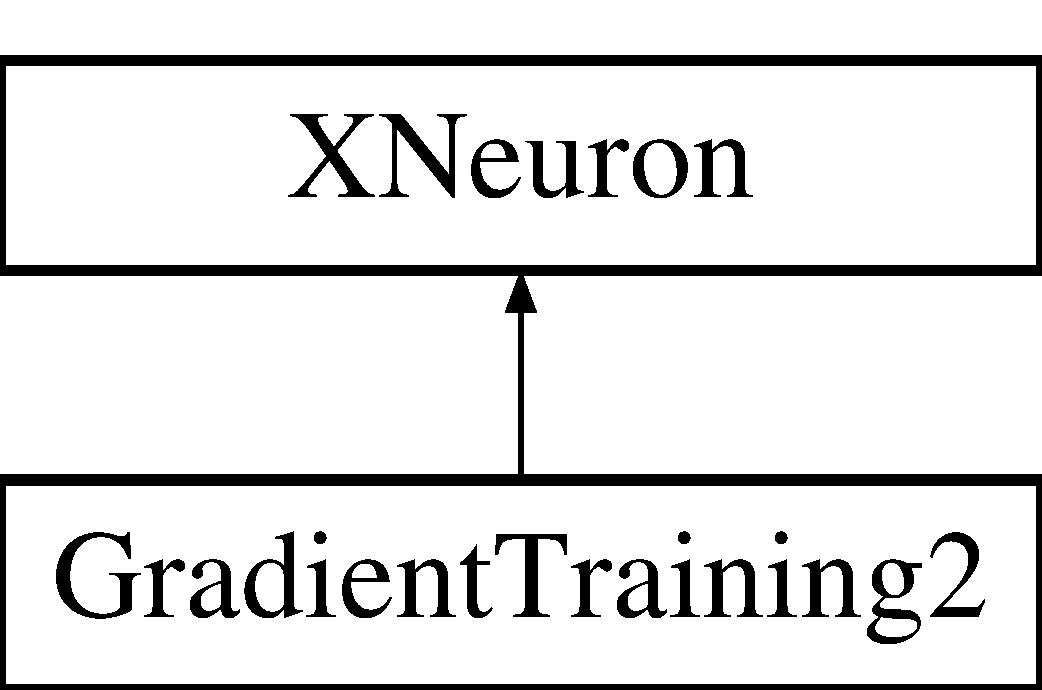
\includegraphics[height=2.000000cm]{class_gradient_training2}
\end{center}
\end{figure}
\subsection*{Public Member Functions}
\begin{DoxyCompactItemize}
\item 
\hypertarget{class_gradient_training2_ad038e32c7301f619c678153af1501e2b}{}\label{class_gradient_training2_ad038e32c7301f619c678153af1501e2b} 
bool {\bfseries train} (Q\+List$<$ Q\+List$<$ bool $>$$>$ \&input, Q\+List$<$ bool $>$ \&m\+Output\+Required)
\item 
\hypertarget{class_gradient_training2_a717d68fa1bd96dcb22b7c4595641f82b}{}\label{class_gradient_training2_a717d68fa1bd96dcb22b7c4595641f82b} 
bool {\bfseries train} (Q\+List$<$ Q\+List$<$ double $>$$>$ \&input, Q\+List$<$ double $>$ \&m\+Output\+Required, Activity\+Function\+::\+Act\+Function)
\item 
\hypertarget{class_gradient_training2_a415863710264644934497a55800ca95e}{}\label{class_gradient_training2_a415863710264644934497a55800ca95e} 
void {\bfseries set\+Input} (const Q\+List$<$ double $>$ \&input)
\item 
\hypertarget{class_gradient_training2_a9a6476c0bbd858a4a699994b4791298f}{}\label{class_gradient_training2_a9a6476c0bbd858a4a699994b4791298f} 
void {\bfseries set\+Input} (const Q\+List$<$ bool $>$ \&input)
\item 
\hypertarget{class_gradient_training2_a261483e252104c75c67ab4a5cecbb002}{}\label{class_gradient_training2_a261483e252104c75c67ab4a5cecbb002} 
double {\bfseries CalcN} (double N)
\end{DoxyCompactItemize}
\subsection*{Additional Inherited Members}


The documentation for this class was generated from the following files\+:\begin{DoxyCompactItemize}
\item 
Gradiente\+Training2.\+h\item 
Gradiente\+Training2.\+cpp\end{DoxyCompactItemize}

\hypertarget{class_online_training}{}\section{Online\+Training Class Reference}
\label{class_online_training}\index{Online\+Training@{Online\+Training}}
Inheritance diagram for Online\+Training\+:\begin{figure}[H]
\begin{center}
\leavevmode
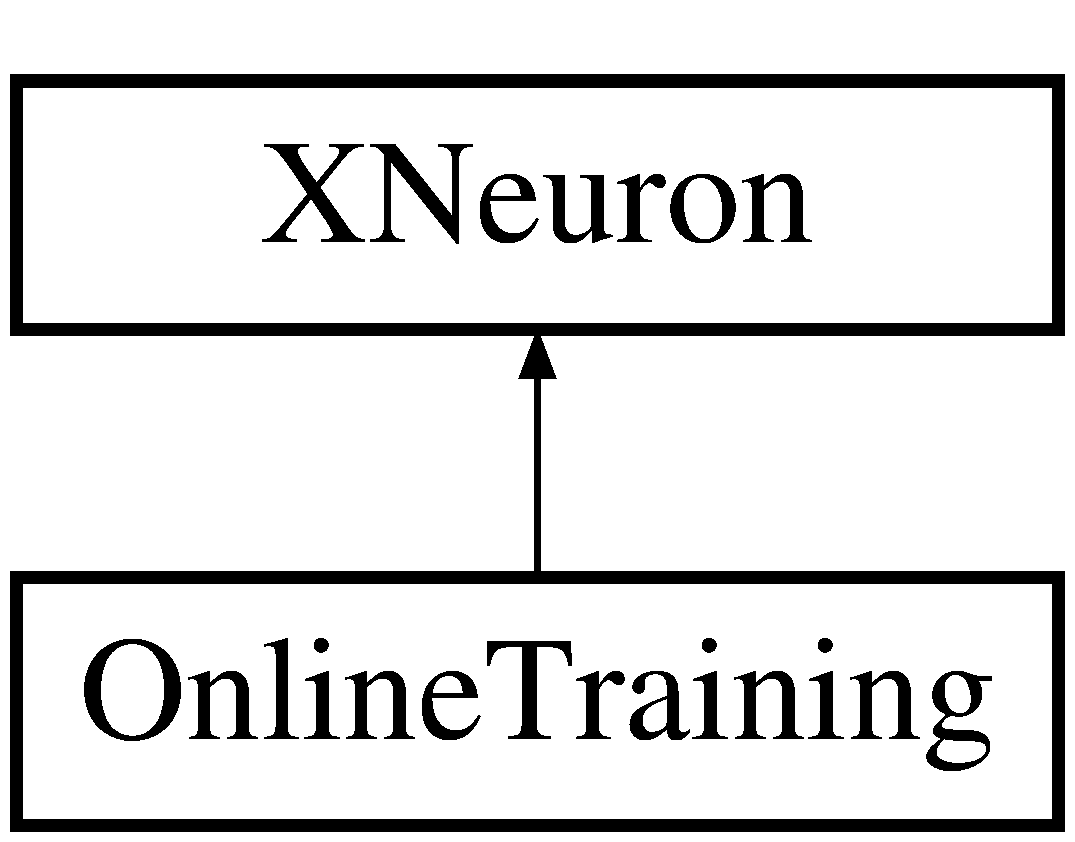
\includegraphics[height=2.000000cm]{class_online_training}
\end{center}
\end{figure}
\subsection*{Public Member Functions}
\begin{DoxyCompactItemize}
\item 
\hypertarget{class_online_training_a70f7c77023c742884f80bed13af05db4}{}\label{class_online_training_a70f7c77023c742884f80bed13af05db4} 
bool {\bfseries train} (Q\+List$<$ Q\+List$<$ bool $>$$>$ \&input, Q\+List$<$ bool $>$ \&m\+Output\+Required)
\item 
\hypertarget{class_online_training_aca19870825ac3f0c35ebdc7583f5571e}{}\label{class_online_training_aca19870825ac3f0c35ebdc7583f5571e} 
bool {\bfseries train} (Q\+List$<$ Q\+List$<$ double $>$$>$ \&input, Q\+List$<$ double $>$ \&m\+Output\+Required, Activity\+Function\+::\+Act\+Function)
\end{DoxyCompactItemize}
\subsection*{Additional Inherited Members}


The documentation for this class was generated from the following files\+:\begin{DoxyCompactItemize}
\item 
Online\+Training.\+h\item 
Online\+Training.\+cpp\end{DoxyCompactItemize}

\hypertarget{class_x_neuron}{}\section{X\+Neuron Class Reference}
\label{class_x_neuron}\index{X\+Neuron@{X\+Neuron}}
Inheritance diagram for X\+Neuron\+:\begin{figure}[H]
\begin{center}
\leavevmode
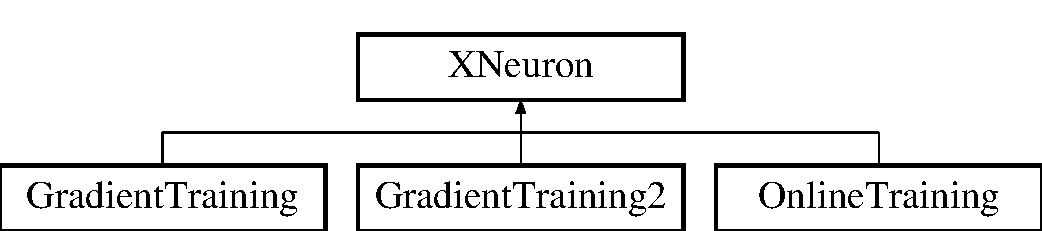
\includegraphics[height=2.000000cm]{class_x_neuron}
\end{center}
\end{figure}
\subsection*{Public Member Functions}
\begin{DoxyCompactItemize}
\item 
\hypertarget{class_x_neuron_ac5616106c0fbf7c527d724b6998c1277}{}\label{class_x_neuron_ac5616106c0fbf7c527d724b6998c1277} 
virtual bool {\bfseries train} (Q\+List$<$ Q\+List$<$ bool $>$$>$ \&input, Q\+List$<$ bool $>$ \&m\+Output\+Required)
\item 
\hypertarget{class_x_neuron_a02e6eed23c4b1d131d2f0fcc2bc358e6}{}\label{class_x_neuron_a02e6eed23c4b1d131d2f0fcc2bc358e6} 
virtual bool {\bfseries train} (Q\+List$<$ Q\+List$<$ double $>$$>$ \&input, Q\+List$<$ double $>$ \&m\+Output\+Required, Activity\+Function\+::\+Act\+Function)
\item 
\hypertarget{class_x_neuron_ac76b3d3ca7fad9a880b83fa5714e1705}{}\label{class_x_neuron_ac76b3d3ca7fad9a880b83fa5714e1705} 
virtual double {\bfseries output} () const
\item 
\hypertarget{class_x_neuron_a7a6306e0dc045f27136252f84870abb7}{}\label{class_x_neuron_a7a6306e0dc045f27136252f84870abb7} 
virtual bool {\bfseries output\+Binary} () const
\item 
\hypertarget{class_x_neuron_a54ef9c2ed729e21641a967d62c956f91}{}\label{class_x_neuron_a54ef9c2ed729e21641a967d62c956f91} 
virtual double {\bfseries output} (Activity\+Function\+::\+Act\+Function x\+Func) const
\item 
\hypertarget{class_x_neuron_aba98d98aaf1e1027239824d19b3797aa}{}\label{class_x_neuron_aba98d98aaf1e1027239824d19b3797aa} 
virtual Q\+List$<$ double $>$ {\bfseries input} () const
\item 
\hypertarget{class_x_neuron_a0ff6275e2532503c795f77e165b59784}{}\label{class_x_neuron_a0ff6275e2532503c795f77e165b59784} 
virtual void {\bfseries set\+Input} (bool A, bool B)
\item 
\hypertarget{class_x_neuron_a6c1a40a9a965fa2e3ae34988b048014b}{}\label{class_x_neuron_a6c1a40a9a965fa2e3ae34988b048014b} 
virtual void {\bfseries set\+Input} (const Q\+List$<$ bool $>$ \&input)
\item 
\hypertarget{class_x_neuron_a16c2071b13ca0e25e88bfa113881d489}{}\label{class_x_neuron_a16c2071b13ca0e25e88bfa113881d489} 
virtual void {\bfseries set\+Input} (const Q\+List$<$ double $>$ \&input)
\item 
\hypertarget{class_x_neuron_a353abf29fecd904cbdbae031b99f5d23}{}\label{class_x_neuron_a353abf29fecd904cbdbae031b99f5d23} 
virtual void {\bfseries init\+Weight} (const Q\+List$<$ bool $>$ \&input)
\item 
\hypertarget{class_x_neuron_a57c9fa808e03d27c96edc9d7774534ce}{}\label{class_x_neuron_a57c9fa808e03d27c96edc9d7774534ce} 
virtual void {\bfseries Reset\+Weight} (const Q\+List$<$ bool $>$ \&input)
\item 
\hypertarget{class_x_neuron_a49794575e12094f4f336909a788b5d03}{}\label{class_x_neuron_a49794575e12094f4f336909a788b5d03} 
virtual void {\bfseries init\+Weight} (const Q\+List$<$ double $>$ \&input)
\item 
\hypertarget{class_x_neuron_a05efde6b330a87218eb9560b93837142}{}\label{class_x_neuron_a05efde6b330a87218eb9560b93837142} 
virtual void {\bfseries Reset\+Weight} (const Q\+List$<$ double $>$ \&input)
\item 
\hypertarget{class_x_neuron_a963745b2b34d5bcfe21be3a81a0b7c18}{}\label{class_x_neuron_a963745b2b34d5bcfe21be3a81a0b7c18} 
virtual Q\+List$<$ double $>$ {\bfseries weight} () const
\item 
\hypertarget{class_x_neuron_a46b611c44bfd8c9ca391a8c55698ca5e}{}\label{class_x_neuron_a46b611c44bfd8c9ca391a8c55698ca5e} 
virtual void {\bfseries set\+Weight} (double A, double B)
\item 
\hypertarget{class_x_neuron_ab91134205006e82b872d9724bc677106}{}\label{class_x_neuron_ab91134205006e82b872d9724bc677106} 
virtual void {\bfseries set\+Weight} (double A, double B, double C)
\item 
\hypertarget{class_x_neuron_a80505d7f586c511cbc79646788ab2f22}{}\label{class_x_neuron_a80505d7f586c511cbc79646788ab2f22} 
virtual void {\bfseries set\+Weight} (const Q\+List$<$ double $>$ \&weight)
\item 
\hypertarget{class_x_neuron_a07b4676157782cfed59364c91cf84aed}{}\label{class_x_neuron_a07b4676157782cfed59364c91cf84aed} 
virtual double {\bfseries bias} () const
\item 
\hypertarget{class_x_neuron_aeaf8310866462df8946df4b2c65e306a}{}\label{class_x_neuron_aeaf8310866462df8946df4b2c65e306a} 
virtual void {\bfseries Calc\+Output} ()
\item 
\hypertarget{class_x_neuron_a8b3849d0c889f676ec3f1863167aadec}{}\label{class_x_neuron_a8b3849d0c889f676ec3f1863167aadec} 
void {\bfseries set\+Weight} (double A, double B, double C, double D)
\end{DoxyCompactItemize}
\subsection*{Public Attributes}
\begin{DoxyCompactItemize}
\item 
\hypertarget{class_x_neuron_aba949156bcc9aa4a0d84c342bf8b5bf4}{}\label{class_x_neuron_aba949156bcc9aa4a0d84c342bf8b5bf4} 
Q\+List$<$ \hyperlink{class_x_neuron}{X\+Neuron} $>$ {\bfseries m\+Next\+Neuron}
\end{DoxyCompactItemize}
\subsection*{Protected Attributes}
\begin{DoxyCompactItemize}
\item 
\hypertarget{class_x_neuron_ac69d818c1d38c321a232fd9557635300}{}\label{class_x_neuron_ac69d818c1d38c321a232fd9557635300} 
Q\+List$<$ double $>$ {\bfseries m\+Input}
\item 
\hypertarget{class_x_neuron_abaffc1446ad83470d54c87de5a6a117a}{}\label{class_x_neuron_abaffc1446ad83470d54c87de5a6a117a} 
double {\bfseries m\+Output} = 0
\item 
\hypertarget{class_x_neuron_af4b92137a421c14961971e24ced0f458}{}\label{class_x_neuron_af4b92137a421c14961971e24ced0f458} 
double {\bfseries m\+Bias} = 0
\item 
\hypertarget{class_x_neuron_a7b9457385c80f6ec33dd301b7f071700}{}\label{class_x_neuron_a7b9457385c80f6ec33dd301b7f071700} 
Activity\+Function\+::\+Act\+Function {\bfseries m\+Func}
\item 
\hypertarget{class_x_neuron_a62fecf6b44a6c56f983e20591fa62404}{}\label{class_x_neuron_a62fecf6b44a6c56f983e20591fa62404} 
Q\+List$<$ double $>$ {\bfseries m\+Weight}
\end{DoxyCompactItemize}


The documentation for this class was generated from the following files\+:\begin{DoxyCompactItemize}
\item 
xneuron.\+h\item 
xneuron.\+cpp\end{DoxyCompactItemize}

%--- End generated contents ---

% Index
\backmatter
\newpage
\phantomsection
\clearemptydoublepage
\addcontentsline{toc}{chapter}{Index}
\printindex

\end{document}
